\documentclass[a4paper,11pt,twoside]{report}
% THIS FILE SHOULD BE COMPILED BY pdfLaTeX

% ----------------------   PREAMBLE PART ------------------------------

% ------------------------ ENCODING & LANGUAGES ----------------------

\usepackage[utf8]{inputenc}
\usepackage[MeX]{polski} % Not needed unless You have a name with polish symbols or sth (doesn't work, maybe it works:)

\usepackage[T1]{fontenc}
\usepackage[english, polish]{babel}


\usepackage{amsmath, amsfonts, amsthm, latexsym} % MOSTLY MATHEMATICAL SYMBOLS

\usepackage[final]{pdfpages} % INPUTING TITLE PDF PAGE - GENERATE IT FIRST!
\usepackage{biblatex}
\addbibresource{../references/bibliography.bib}

\usepackage{commath} % various commands which can make writing math expressions easier --- documentation available at: https://ctan.gust.org.pl/tex-archive/macros/latex/contrib/commath/commath.pdf

\usepackage[hidelinks]{hyperref} % for hyperlinks, for example, urls, references to equations, entries in a bibliography --- hidelinks option removes rectangles around hiperlinks


% ---------------- MARGINS, INDENTATION, LINESPREAD ------------------

\usepackage[inner=20mm, outer=20mm, bindingoffset=10mm, top=25mm, bottom=25mm]{geometry} % MARGINS


\linespread{1.5}
\allowdisplaybreaks         % ALLOWS BREAKING PAGE IN MATH MODE

\usepackage{indentfirst}    % IT MAKES THE FIRST PARAGRAPH INDENTED; NOT NEEDED
\setlength{\parindent}{5mm} % WIDTH OF AN INDENTATION


%---------------- RUNNING HEAD - CHAPTER NAMES, PAGE NUMBERS ETC. -------------------

\usepackage{fancyhdr}
\pagestyle{fancy}
\fancyhf{}
% PAGINATION: LEFT ALIGNMENT ON EVEN PAGES, RIGHT ALIGNMENT ON ODD PAGES 
\fancyfoot[LE,RO]{\thepage} 
% RIGHT HEADER: zawartość \rightmark do lewego, wewnętrznego (marginesu) 
\fancyhead[LO]{\sc \nouppercase{\rightmark}}
% lewa pagina: zawartość \leftmark do prawego, wewnętrznego (marginesu) 
\fancyhead[RE]{\sc \leftmark}

\renewcommand{\chaptermark}[1]{\markboth{\thechapter.\ #1}{}}

% HEAD RULE - IT'S A LINE WHICH SEPARATES HEADER AND FOOTER FROM CONTENT
\renewcommand{\headrulewidth}{0 pt} % 0 MEANS NO RULE, 0.5 MEANS FINE RULE, THE BIGGER VALUE THE THICKER RULE


\fancypagestyle{plain}{
  \fancyhf{}
  \fancyfoot[LE,RO]{\thepage}
  
  \renewcommand{\headrulewidth}{0pt}
  \renewcommand{\footrulewidth}{0.0pt}
}
\usepackage{float}
\usepackage{multirow}
\usepackage{caption}
\usepackage{subcaption}
\usepackage{forest}
\usepackage[T1]{fontenc}
\usepackage[polish]{babel}
\usepackage[utf8]{inputenc}



% --------------------------- CHAPTER HEADERS ---------------------

\usepackage{titlesec}
\titleformat{\chapter}
  {\normalfont\Large \bfseries}
  {\thechapter.}{1ex}{\Large}

\titleformat{\section}
  {\normalfont\large\bfseries}
  {\thesection.}{1ex}{}
\titlespacing{\section}{0pt}{30pt}{20pt} 

    
\titleformat{\subsection}
  {\normalfont \bfseries}
  {\thesubsection.}{1ex}{}


% ----------------------- TABLE OF CONTENTS SETUP ---------------------------

\def\cleardoublepage{\clearpage\if@twoside
\ifodd\c@page\else\hbox{}\thispagestyle{empty}\newpage
\if@twocolumn\hbox{}\newpage\fi\fi\fi}


% THIS MAKES DOTS IN TOC FOR CHAPTERS
\usepackage{etoolbox}
\makeatletter
\patchcmd{\l@chapter}
  {\hfil}
  {\leaders\hbox{\normalfont$\m@th\mkern \@dotsep mu\hbox{.}\mkern \@dotsep mu$}\hfill}
  {}{}
\makeatother

\usepackage{titletoc}
\makeatletter
\titlecontents{chapter}% <section-type>
  [0pt]% <left>
  {}% <above-code>
  {\bfseries \thecontentslabel.\quad}% <numbered-entry-format>
  {\bfseries}% <numberless-entry-format>
  {\bfseries\leaders\hbox{\normalfont$\m@th\mkern \@dotsep mu\hbox{.}\mkern \@dotsep mu$}\hfill\contentspage}% <filler-page-format>

\titlecontents{section}
  [1em]
  {}
  {\thecontentslabel.\quad}
  {}
  {\leaders\hbox{\normalfont$\m@th\mkern \@dotsep mu\hbox{.}\mkern \@dotsep mu$}\hfill\contentspage}

\titlecontents{subsection}
  [2em]
  {}
  {\thecontentslabel.\quad}
  {}
  {\leaders\hbox{\normalfont$\m@th\mkern \@dotsep mu\hbox{.}\mkern \@dotsep mu$}\hfill\contentspage}
\makeatother



% ---------------------- TABLES AD FIGURES NUMBERING ----------------------

\renewcommand*{\thetable}{\arabic{chapter}.\arabic{table}}
\renewcommand*{\thefigure}{\arabic{chapter}.\arabic{figure}}


% ------------- DEFINING ENVIRONMENTS FOR THEOREMS, DEFINITIONS ETC. ---------------

\makeatletter
\newtheoremstyle{definition}
{3ex}%                           % Space above
{3ex}%                           % Space below
{\upshape}%                      % Body font
{}%                              % Indent amount
{\bfseries}%                     % Theorem head font
{.}%                             % Punctuation after theorem head
{.5em}%                          % Space after theorem head, ' ', or \newline
{\thmname{#1}\thmnumber{ #2}\thmnote{ (#3)}}
\makeatother

\theoremstyle{definition}
\newtheorem{theorem}{Theorem}[chapter]
\newtheorem{lemma}[theorem]{Lemma}
\newtheorem{example}[theorem]{Example}
\newtheorem{proposition}[theorem]{Proposition}
\newtheorem{corollary}[theorem]{Corollary}
\newtheorem{definition}[theorem]{Definition}
\newtheorem{remark}[theorem]{Remark}

% -------------------------- USER SETTINGS ---------------------------

\newcommand{\tytul}{Nowoczesne modelowanie krzywej dochodowości z dynamicznymi czynnikami makroekonomicznymi}

\renewcommand{\title}{Modern Yield Curve Modeling with Dynamic Macroeconomic Factors\\
An Econometric Extension Benchmarked Against Hull-White Stochastic Methods }
\newcommand{\type}{Master} % Master OR Engineer
\newcommand{\supervisor}{dr Marcin Bielecki} % TITLE AND NAME OF THE SUPERVISOR


% --------------------- END OF PREAMBLE PART (MOSTLY) --------------------------


% -------------------- DOCUMENT -----------------------

\begin{document}

\sloppy
\selectlanguage{english}

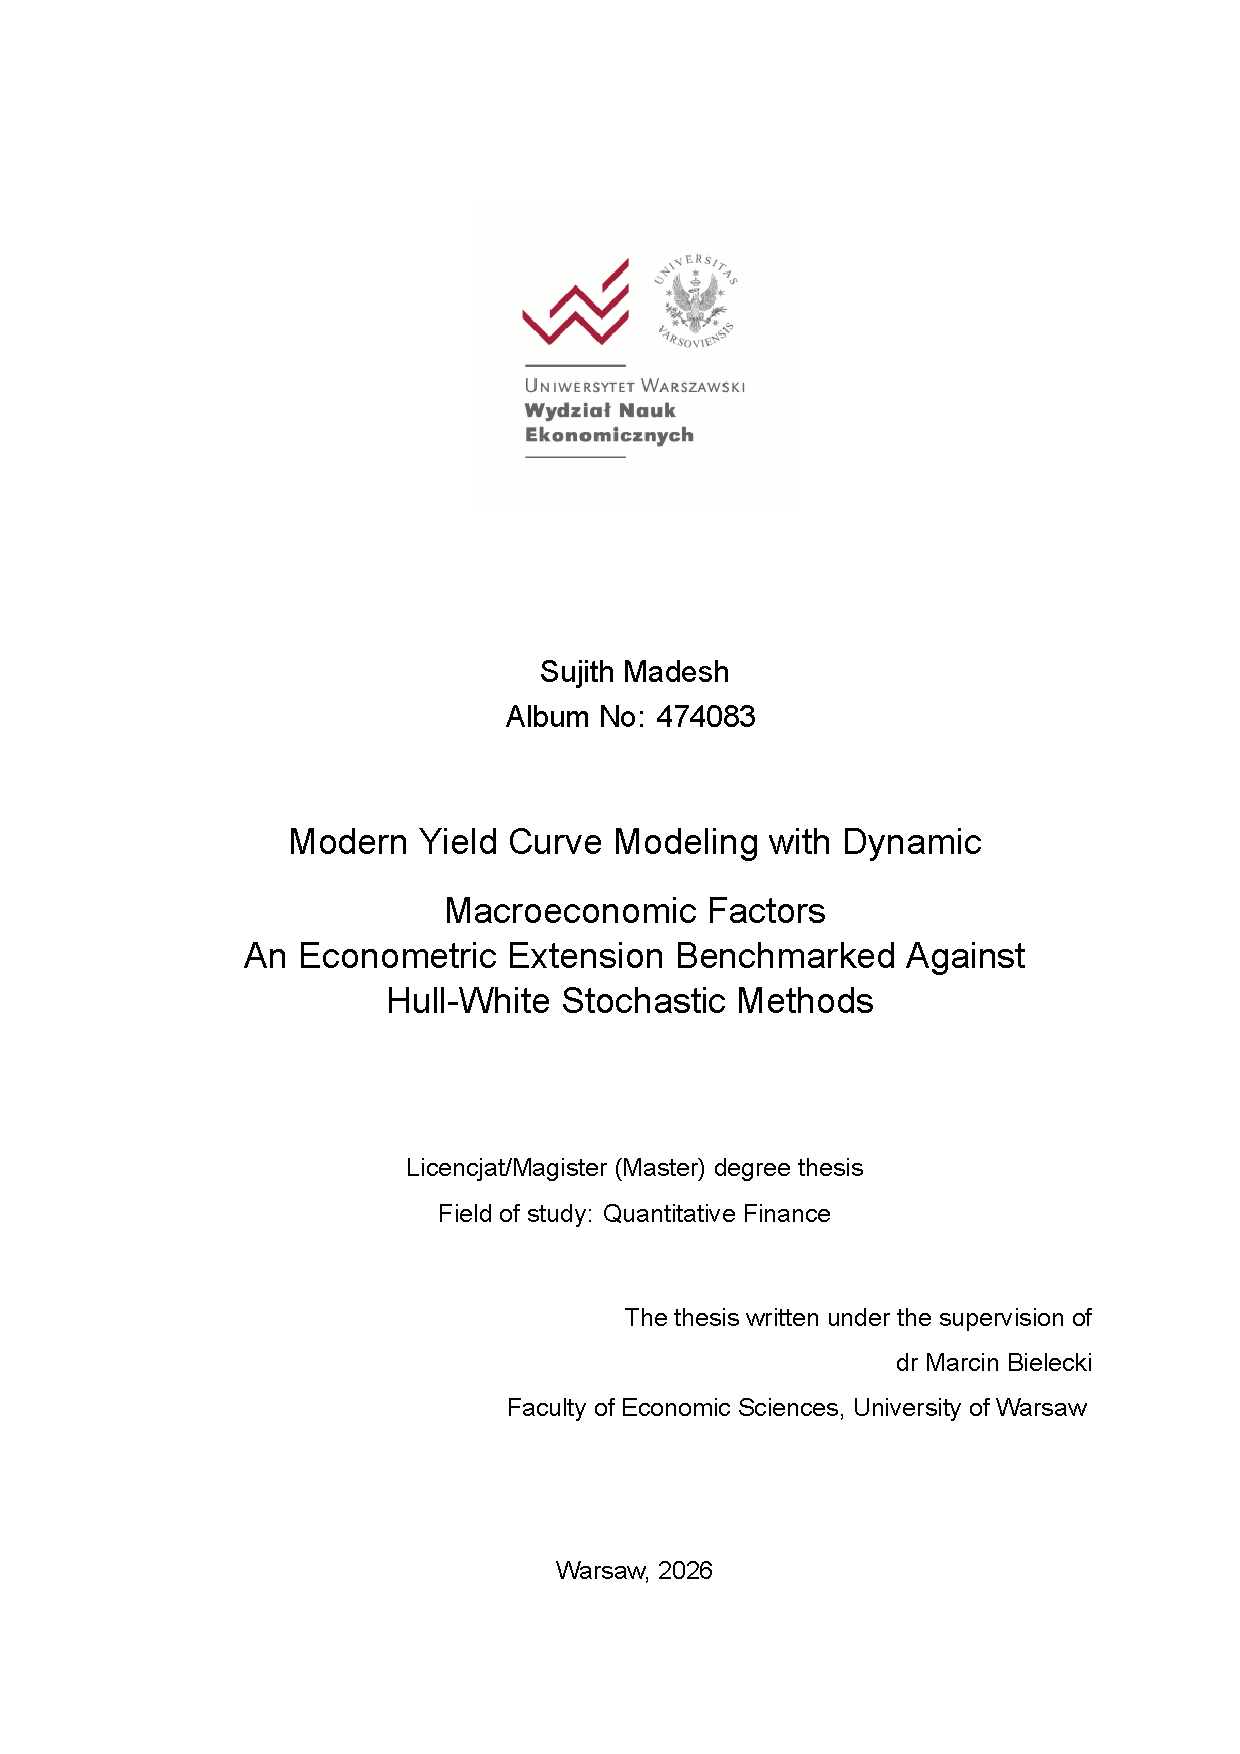
\includepdf[pages=-]{titlepage-en} % THIS INPUTS THE TITLE PAGE

% \null\thispagestyle{empty}\newpage

% ---------- FRONT MATTER ----------
{  \fontsize{12}{14} \selectfont
\begin{abstract}

\begin{center}
\title
\end{center}
The thesis concerns modern yield curve modeling in the presence of changing macroeconomic
conditions. The analysis covers parametric representations of the term structure of interest
rates and their dynamic behavior over time. Special attention is given to the relationship
between yield curve factors and selected macroeconomic variables such as inflation, economic
activity, and monetary policy indicators. Econometric approaches integrating macro-financial
information are discussed alongside stochastic short-rate models commonly applied in financial
practice. The study presents a comparative perspective on the ability of different modeling
frameworks to describe yield curve dynamics and economic interpretation under varying market
conditions.

\vspace{0.5cm}

\begin{center}
\textbf{Key words:}\\
yield curve, term structure, macroeconomic factors, nelson--siegel model, hull--white model, econometric modeling
\end{center}
\end{abstract}

% \null\thispagestyle{empty}\newpage


{\selectlanguage{polish} \fontsize{12}{14}\selectfont
\begin{abstract}

\begin{center}
\tytul
\end{center}

% czas od ostatniego reco

\end{abstract}
}

% \selectlanguage{english} - for English
\tableofcontents
\thispagestyle{empty}


% -------------------- THE BODY OF THE THESIS --------------------------------

\null\thispagestyle{empty}\newpage
\setcounter{page}{3}
\addtocontents{toc}{\protect\thispagestyle{empty}}

\chapter{Introduction}


\section{Motivation}
The term structure of interest rates, commonly referred to as the yield curve, is a fundamental object in finance and macroeconomics. It summarizes market expectations about future interest rates, inflation, and economic conditions, and serves as a key input for asset pricing, portfolio allocation, and risk management. For policymakers, the yield curve provides valuable information about the stance of monetary policy and expectations about future economic activity, while for financial institutions it is central to valuation, hedging, and profitability analysis.

A large body of literature has proposed models to describe and forecast the yield curve. Parametric models such as the Nelson–Siegel and Nelson–Siegel–Svensson specifications offer a parsimonious and intuitive representation of the yield curve through a small number of latent factors. In parallel, stochastic interest rate models, such as the Hull–White model, are widely used in practice due to their analytical tractability and suitability for derivative pricing. Despite their popularity, these frameworks often rely primarily on yield curve information and treat macroeconomic conditions only implicitly, if at all.

Recent empirical evidence suggests that macroeconomic variables—such as inflation, output growth, and monetary policy rates—play a significant role in shaping the dynamics of the yield curve. Ignoring these factors may limit traditional models' ability to explain yield movements and produce accurate forecasts, particularly during periods of economic stress or structural change. This observation motivates integrating macroeconomic information into yield curve modeling frameworks.

\section{Research Objectives and Questions}
The primary objective of this thesis is to examine whether yield curve models that explicitly incorporate macroeconomic factors provide improved explanatory power and forecasting performance compared to standard stochastic interest rate models. To address this objective, the study focuses on the following research questions:

- To what extent do macroeconomic variables explain the dynamics of the latent factors of the yield curve?
- Does a macro-augmented econometric yield curve model outperform the Hull–White one-factor model in terms of in-sample fit and out-of-sample forecasting accuracy?
- How do the two modeling approaches differ in their economic interpretability and response to macroeconomic shocks?

By answering these questions, the thesis aims to assess the practical relevance of macro-financial integration in yield curve modeling.


\section{Contribution of the Thesis}
This thesis contributes to the existing literature in three main ways. First, it extends a widely used yield curve modeling framework by linking its latent factors to observable macroeconomic variables using econometric methods. Second, it provides a direct empirical comparison between a macro-augmented yield curve model and the Hull–White stochastic interest rate model, which remains a standard benchmark in financial practice. Third, the study offers insights into the economic interpretation of yield curve movements by explicitly relating them to macroeconomic conditions.

The results of this research are relevant for both academics and practitioners, particularly in the context of monetary policy analysis, interest rate forecasting, and financial risk management.


\chapter{Literature Review}

\section{Classical Yield Curve Models}

The modeling of the term structure of interest rates has long been a central topic in financial
economics. A seminal contribution is the parametric framework proposed by
\textcite{nelson_siegel_1987}, which represents the yield curve using a small number of latent
factors associated with its level, slope, and curvature. The main advantages of this approach
are its parsimony, flexibility, and economic interpretability, which have led to its widespread
use in empirical research and policy institutions.

An important extension was introduced by \textcite{svensson_1994}, who augmented the
original specification with an additional curvature component to improve the fit at longer
maturities. The Nelson--Siegel--Svensson formulation has since become a standard tool for
estimating sovereign yield curves, particularly in central bank applications. Despite their
success in fitting the cross-sectional shape of the yield curve, these static specifications do
not explicitly capture the dynamic evolution of interest rates.

A dynamic interpretation of the Nelson--Siegel framework was provided by
\textcite{diebold_li_2006}, who demonstrated that the latent yield curve factors can be modeled
as time series processes. Their work established a connection between yield curve modeling
and factor-based forecasting methods and laid the foundation for subsequent macro-financial
extensions.

\section{Macroeconomic Influences on the Yield Curve}

A growing body of literature emphasizes the role of macroeconomic fundamentals in shaping
yield curve dynamics. Early empirical evidence suggests that variables such as inflation,
economic activity, and monetary policy expectations are closely related to movements in yields
across maturities. Models that abstract from these relationships may therefore provide an
incomplete description of interest rate behavior.

\textcite{ang_piazzesi_2003} proposed a no-arbitrage framework that integrates
macroeconomic variables into term structure modeling. Their results show that macroeconomic
shocks significantly affect the entire yield curve, highlighting the importance of incorporating
information from the real economy.

Further contributions demonstrate that yield curve factors themselves contain information
about future macroeconomic conditions. \textcite{diebold_rudebusch_aruoba_2006}
developed a macro-finance model that jointly describes macroeconomic variables and yield
curve factors within a unified dynamic system. Their findings reveal strong interactions
between the level and slope of the yield curve and key macroeconomic indicators, reinforcing
the view that financial and macroeconomic dynamics are closely interconnected.

\section{Econometric Approaches to Yield Curve Dynamics}

Econometric methods such as Vector Autoregression (VAR) and Dynamic Factor Models (DFM)
are widely employed to analyze the joint dynamics of yield curve factors and macroeconomic
variables. VAR models allow for flexible dynamic interactions without imposing strong
structural assumptions, making them particularly suitable for empirical macro-finance
applications.

Dynamic factor models, as discussed by \textcite{stock_watson_2002}, provide a parsimonious
representation of information contained in large macroeconomic datasets by summarizing
co-movements through a small number of latent factors. When applied to yield curve modeling,
these approaches offer a natural framework for integrating macroeconomic information into
interest rate dynamics.

Empirical studies indicate that macro-augmented yield curve models often outperform
purely yield-based specifications in forecasting exercises, particularly at medium and long
horizons \parencite{koop_korobilis_2010}. At the same time, these models maintain a relatively
transparent economic interpretation, which is desirable for policy analysis and financial risk
management.

\section{Stochastic Interest Rate Models}

An alternative strand of the literature focuses on stochastic models of interest rates, with
particular emphasis on applications in pricing and risk management. Short-rate models
describe the evolution of an instantaneous interest rate from which the entire term structure
can be derived. Among these, the Hull--White one-factor model remains one of the most widely
used frameworks in practice.

\textcite{hull_white_1990} extended earlier mean-reverting short-rate models by allowing for
time-dependent parameters, enabling an exact fit to the observed initial yield curve. The
analytical tractability of the model and its suitability for pricing interest rate derivatives
have contributed to its widespread adoption in financial institutions. However, the model
abstracts from explicit macroeconomic mechanisms and relies primarily on market-implied
interest rate dynamics.

Due to these characteristics, stochastic short-rate models are commonly used as benchmarks
when evaluating alternative yield curve modeling approaches, particularly those aimed at
improving economic interpretation rather than pricing accuracy.

\section{Summary and Research Gap}

The literature reveals two dominant approaches to yield curve modeling. The first emphasizes
econometric representations of yield curve factors and their relationship with macroeconomic
variables, while the second focuses on stochastic interest rate models designed primarily for
pricing and risk management. Although both strands have been extensively studied, direct
empirical comparisons between macro-augmented econometric yield curve models and
stochastic short-rate models using a consistent dataset and evaluation framework remain
relatively limited.

This thesis addresses this gap by integrating macroeconomic variables into an econometric
yield curve model and benchmarking its performance against the Hull--White stochastic model.

\chapter{Methodology}

\section{Yield Curve Estimation}
% Nelson--Siegel equations

\section{Macroeconomic Extension}
% VAR / DFM structure

\section{Stochastic Benchmark Model}
% Hull--White SDE

\section{Model Evaluation Criteria}
% RMSE, forecasting

\chapter{Data}

\section{Bond Yield Data}
% Source, frequency, maturities

\section{Macroeconomic Variables}
% Inflation, GDP, policy rates

\section{Data Transformations}
% Stationarity, scaling

\chapter{Empirical Results}

\section{Yield Curve Fit}
% In-sample fit

\section{Forecasting Performance}
% Out-of-sample results

\section{Macroeconomic Sensitivity}
% Impulse responses

\chapter{Conclusion}

\section{Summary of Findings}
% Key results

\section{Limitations}
% What could be improved

\section{Further Research}
% Extensions


% ---------- BIBLIOGRAPHY ----------
\cleardoublepage
\printbibliography

% ---------- APPENDICES ----------
\cleardoublepage
\appendix
\chapter{Additional Tables and Figures}

% Extra material here


\end{document}
